\documentclass[10pt,letterpaper,twocolumn]{article}

%2012-10-01 - Document préparé par David Lafrenière, pour le cours PHY3040.

%Pour langue et caractères spéciaux
\usepackage[french]{babel} 
\usepackage[T1]{fontenc}
\usepackage{lmodern}
\usepackage[utf8]{inputenc}

\usepackage[backend=biber, style=nature]{biblatex}
\addbibresource{reference.bib}
  
%Package for math expression
\usepackage{amsmath}
\usepackage{amsthm,amstext,amsfonts,bm,amssymb,amsthm}
\usepackage{mathtools}
\usepackage{bm}
\usepackage{gensymb}
\usepackage{mathrsfs}
\usepackage{physics}
\usepackage{chemgreek, mhchem}
\usepackage{nicefrac}

%Package for drawings
\usepackage{tikz}
\usetikzlibrary{calc,patterns,angles,quotes}
\usepackage[compat=1.1.0]{tikz-feynman}
%\usetikzlibrary{3d}
\usetikzlibrary{decorations.pathreplacing}
\usetikzlibrary{automata,positioning}
%\usepackage{lineno}

%Package pour les symbole astronomiques
%\usepackage{wasysym}

\usepackage{hyperref}

%Pour ajuster les marges
\usepackage[top=2cm, bottom=2cm, left=2cm, right=2cm, columnsep=20pt]{geometry}

% Pour la commande onecolabstract (résumé 1 pleine largeur)
\usepackage{abstract}
	\renewcommand{\abstractnamefont}{\normalfont\bfseries}
	\renewcommand{\abstracttextfont}{\normalfont\itshape}

% Pour les titres de section/sous-section
\usepackage[compact]{titlesec}
\titleformat{\section}{\large\bfseries}{\thesection}{1em}{}
\titleformat{\subsection}{\normalsize\bfseries}{\thesubsection}{1em}{}
\titleformat{\subsubsection}{\normalsize}{\thesubsubsection}{1em}{}

%Package for graphic expression
\usepackage{graphicx}
\usepackage{wrapfig}
\usepackage{float}
\usepackage{caption}
\usepackage{subcaption}
\usepackage{enumitem}
\usepackage{multirow}

%Shorthand for space and some math expressions
\newcommand{\s}{\hspace{0.1cm}}
\renewcommand{\Im}{\operatorname{\mathbb{I}m}}
\renewcommand{\Re}{\operatorname{\mathbb{R}}}
%Shorthand for partial differential
\newcommand{\partialD}[2]{\frac{\partial #1}{\partial #2}}
%Shorthand for \left(\right)
\DeclarePairedDelimiter\autobracket{(}{)}
\newcommand{\br}[1]{\autobracket*{#1}}

\newcommand{\unit}[1]{\hspace{0.15cm}\text{#1}}
\newcommand{\pyoutput}[2]{#2} % Simply output #2, use #1 as tag for python reader

%Pour inclure des adresse web
\usepackage{url}

%Titre
\title{\vspace{-10mm}\Large
Diffusion Raman %%%***éditer cette ligne***
\vspace{-4mm}}

%Auteur
\author{\large
Alexandre Adam
}
\date{\vspace{-8mm}}

\captionsetup{labelfont=bf, format=plain, font=footnotesize}

\begin{document}

\twocolumn[
\maketitle
\begin{onecolabstract} % 10 points
	Nous déterminons la nature chimique de trois échantillons à partir de leur spectre Raman dans le champ Stokes. On trouve une raie à $788.0\pm 2\unit{cm}^{-1}$ pour le premier échantillon correspondant au polytope 6H-\ce{SiC}. Les pics $307\pm 5\unit{cm}^{-1}$ et $351 \pm 5\unit{cm}^{-1}$ apparaissent dans le spectre de l'échantillon 2, indiquant la présence de \ce{InP}. Le pic $230 \pm 2\unit{cm}^{-1}$ est observé pour l'échantillon 3, indiquant un crystal de \ce{TiS2}. Nous vérifions aussi la loi de dispersion du spectroscope utilisé en laboratoire, et trouvons que la résolution expérimentale est plus basse que la résolution idéale. Finalement, on mesure la température du souffre après quelques minutes d'expositions au laser comme étant $T = 3.3 \pm 2\s\s 10^2K$, une augmentation de quelques dizaine de degrés par rapport à la température ambiante.
\vspace{4mm} %
\end{onecolabstract}
]

\section{Introduction}\label{intro} % 5 points
La spectroscopie Raman joue un rôle d'importance grandissante dans plusieurs domaines de la science. En 2017, le prix de la Découverte Scientifique de l'année, remis par Québec Science, est remporté par Kevin Petrecca et Frédérick Leblond pour leur sonde à spectroscopie Raman, capable de distinguer un tissu de cerveau sain d'un tissus cancéreux avec une efficacité presque parfaite\footnote{\href{https://www.quebecscience.qc.ca/sciences/les-10-decouvertes-de-2017/2-sonde-anti-cancer/}{Sonde anti-cancer}, \textit{Québec-Science}. (2018)}. Ce type d'avancé met en lumière le rôle cruciale de la spectroscopie Raman pour identifier la structure interne d'un crystal ou d'un tissu organique par ses modes de vibrations internes. \par
Dans ce rapport, on utilise la spectroscopie Raman pour identifier trois échantillons par leur raies Raman dans le champ Stokes. On en profite aussi pour vérifier la relation de dispersion théorique d'un spectroscope en mesurant la largeur d'une raie plasma bien connu provenant de la source laser He-Ne avec une raie principale à $632.8\unit{nm}$. Finalement, on mesure la température d'un crystal de souffre après une exposition au laser de quelques minutes par le rapport d'intensité de ses raies en champ Stokes et anti-Stokes.

\section{Théorie}\label{sec:theorie} % 10 points
La diffusion Raman spontanée est un processus de troisième ordre (3 vertex) dans la théorie des perturbations quantiques\supercite{Yu2010extension}. La Figure \ref{fig:FeynmanD} montre le diagramme de Feynman représentant une diffusion Raman. Le phonon peut être absorbé par l'électron, dans quel cas on parle du champ \textit{anti-Stokes}; il peut aussi être émis par l'électron (champ \textit{Stokes}). \par
Les phonons optiques sont des vibrations du réseau crystallin qui font intervenir des ions de signe opposé. Leur vibration produit un dipôle oscillant et est facilement excité par un faisceau lumineux incident. Ce sont ces phonons qui nous intéressent, puisque leur intensité dans le spectre Raman permet de les distinguer facilement. 

\begin{figure}[H]
	\centering
	\resizebox{!}{5cm}{
	\begin{tikzpicture}
		\tikzfeynmanset{
				every vertex={black, dot}, small
			}
		\begin{feynman}
			\vertex (a) {\large$\hbar \omega_i$};
			\vertex [right=of a] (b);
			\vertex [above right=of b] (c);
			\vertex [below right=of c] (d);
			\vertex [right=of d] (e) {\large$\hbar \omega_s$};
			\vertex [above=of c] (p) {\large$\hbar \omega_p$};
			
			\diagram* {
				(a) -- [photon] (b) -- [fermion, quarter left, edge label=\large$e^-$] (c) -- [fermion, quarter left, edge label=$e^-$] (d) -- [photon] (e);
				(b) -- [charged scalar, edge label'=$\large\text{trou}$, half right] (d);
				(c) -- [photon, edge label=$\large\text{phonon}$] (p);
			};
		\end{feynman}
		\node [below=of a] (t) {\large temps};
		\node [right=of t] (t1) {};
		\draw [->] (t) -- (t1); 
	\end{tikzpicture}
	}
	\caption{Diagramme de Feynman dépictant le processus de diffusion Raman. Un photon (\leadsto) incident d'énergie $\hbar \omega_i$ interagit avec le milieu pour créer une paire électron-trou. Ensuite, un phonon optique est absorbé (anti-Stokes) ou émis (Stokes) par l'électron, qui se recombine avec le trou pour former un nouveau photon d'énergie $\hbar \omega_s = \hbar \omega_i \pm \hbar \omega_p$. }
	\label{fig:FeynmanD}
\end{figure}




\section{Méthodologie}\label{sec:metho} % 15 points

\subsection{Montage}
Pour obtenir les spectres Raman, on utilise le montage dépicté à la Figure \ref{fig:montage}. Le faisceau laser est obtenu par l'excitation d'un plasma He-Ne avec la raie principale (stimulée) ${\lambda_L = 632.816\s nm}$. Le plasma possède plusieurs raies plasma dont la longueur d'onde se situe dans le spectre Stokes. Ces raies ont étés identifiés au début de l'expérience pour calibrer le montage. \par

Les photons diffus par l'effet Raman sont émis dans une direction aléatoire à partir de l'échantillon. La lentille $L_1$ capture ces photons ainsi que les photons du faisceau principal qui ont subis une diffusion Rayleigh. La lentille $L_2$ concentre les photons collectés vers une fente de largeur $\delta x$, où quelques photons ambiants peuvent à ce point entrer dans le spectromètre à réseau double. L'utilisation d'un spectromètre double permet d'attenuer l'intensité de la raie principale diffuse à l'intérieur du spectromètre d'un facteur de $\sim 10^{-10}$, suffisant pour isoler les pics Raman d'une intensité $\gtrsim 10^{-4}$ fois plus faible que la lumière diffuse à l'intérieur du premier spectromètre. Comme le signal est faible, on utilise un photo-multiplicateur GaAs refroidit à $-20^oC$ pour amplifier le signal qui arrive sous forme d'impulsion électrique dans le compteur de photon. \par
Ce montage nous permet de déterminer l'intensité relative d'une raie avec une mesure précise de son énergie (erreur inférieur à $2\unit{cm}^{-1}$). 
\begin{figure}[H]
	\centering
	\resizebox{!}{7cm}{
	\begin{tikzpicture}
		\node (O) at (0, 0) {};
		\node[above right=1cm and 1cm of O, inner sep=0pt] (Laser) {};
		\node[ above right=2cm and 2cm of Laser, inner sep=0pt] (Echantillon) {};
		\node[below right=0.5cm and .5cm of Echantillon, inner sep=0pt] (LaserOut) {};
		\node[below=1cm of Echantillon, inner sep=0pt] (Lentille1) {};
		\node[below=2cm of Lentille1, inner sep=0pt] (Lentille2){};
		\node[below=1cm of Lentille2, inner sep=0pt] (Fente) {};
		\node[below=1.5cm of Fente, inner sep=0pt] (SBottom) {};
		\node[below=.5cm of SBottom, inner sep=0pt] (PM) {};
		\node[below left=.5cm and 1cm of PM, inner sep=0pt] (PMBottom) {};
		\node[left=1cm of PMBottom, inner sep=0pt] (CPS) {};
		\node[right=.75 of Lentille1] {$L_1$};
		\node[right=.75 of Lentille2] {$L_2$};
		
		\draw[rotate around={45:(O)}] (O)++(-1.5cm, -.5cm) rectangle ++(3.17cm, 1cm) node[pos=.5, rotate around={45:(O)}] {Laser He-Ne};
		\draw (Echantillon)++(-1.5, 1) rectangle ++(2, -1) node[pos=.5] {Échantillon};
		\draw[<->] (Lentille1)++(-.5, 0) -- ++(1, 0);
		\draw[<->] (Lentille2)++(-.5, 0) -- ++(1, 0);
		\draw (Fente)++(2cm, 0) rectangle ++(-3cm, -1.5cm) node[pos=.5, text width=3cm, align=center] {Spectromètre \\ double};
		\draw (PM)++(2cm, 0) rectangle ++(-3cm, -1cm) node[pos=.5, text width=3cm, align=center] {Photo- \\ multiplicateur};
		\draw (CPS)++(0, 0.5cm) rectangle ++(-2cm, -1cm) node[pos=.5, text width=3cm, align=center] {Compteur \\ de photon};
		
		\draw (Laser) -- (Echantillon) -- (LaserOut);
		\draw (Echantillon) -- ++(-.5, -1.075) -- ++(0, -2) -- (Fente);
		\draw (Echantillon) -- ++(.5, -1.075) -- ++(0, -2) -- (Fente);
		\draw (SBottom)++(0, .06) -- (PM)++(0, -.11);
		\draw[->] (PMBottom) -- (CPS);
	\end{tikzpicture}
	}	
	\caption{Montage de spectroscopie Raman}
	\label{fig:montage}
\end{figure}
Le spectromètre utilise un réseau avec une densité de trait ${n=1200 \unit{traits}/\text{mm}}$ et une longueur focale ${F=200\unit{mm}}$ (\textit{i.e.} la distance entre le point de sortie et le deuxième miroir concave) pour disperser la lumière. 

\subsection{Relation de dispersion}
On vérifie la loi de dispersion linéaire du spectromètre double en utilisant la raie plasma ${\lambda_p = 692.9\unit{nm}}$ associé à la transition électronique ${3s(J=1) \rightarrow 5p(J=2)}$ de ${\ce{Ne}\s \text{I}}$\supercite{NIST_ASD}. On mesure la largeurs $\delta \lambda$ de cette raie pour 3 largeurs de fente $\delta x$ différentes. Comme on utilise le premier ordre de diffraction (${k=1}$), et que les deux spectromètres sont placés en série, on s'attend à ce que la largeur d'un pic $\delta \lambda$ respecte la loi 
\begin{equation}\label{eq:dispersion}
	\frac{\delta \lambda}{\delta x} = \frac{10^6 \cos \beta}{2nF} \s \s(\text{nm}\s\text{mm}^{-1}),
\end{equation}
où $\beta$ est l'angle du faisceau incident par rapport à la normale du réseau. Dans notre cas, ${\beta = 0}$.

\subsection{Identification des échantillons}

Le pied de la raie principale possède une intensité élevé jusqu'à une énergie de $200\unit{cm}^{-1}$, rendant impossible la mesure du spectre de Brillouin (typiquement autour de quelques cm$^{-1}$ de la raie principale). On se concentre donc sur les phonons optiques des échantillons. On s'intéresse en particulier aux pics générés par l'interaction d'un seul phonon avec un électron. Leur section efficace est plus importante que les processus d'ordre plus grand.
La Table \ref{tab:echantillon} résume les pics distinctifs de la nature possible des différents échantillons qui nous ont permis de les identifiés en laboratoire.
\begin{table}[H]
	\centering
	\caption{Pics Raman attendus}
	\label{tab:echantillon}
	\begin{tabular}{|c|c|c|}
		\hline
		&& Pic Raman [cm$^{-1}$] \\\hline
		\multirow{2}{*}{Échantillon 1} & 4H-\ce{SiC}\supercite{Burton1998}  & $777.0$\\\cline{2-3} 
		     & 	6H-\ce{SiC}\supercite{Burton1998} & $788.0$ \\\hline
		\multirow{2}{*}{Échantillon 2} & \ce{Si}  & 520 \\\cline{2-3} 
		 	 & 	\ce{InP}\supercite{Mooradian1966} & $307 \pm 8$ et $351 \pm 5$\\\hline
 		\multirow{2}{*}{Échantillon 3} & \ce{SnS2}\supercite{Mead1976}  & $317 \pm 1$\\\cline{2-3} 
     		& 	\ce{TiS2}\supercite{Leonelli1980} & $230 \pm 10$ et $345 \pm 10$\\\hline
	\end{tabular}
\end{table}
\subsection{Mesure de la température}
La température d'un échantillon est mesuré à partir du ratio d'intensité d'un pic dans le champ Stokes et son pic correspondant dans le champ anti-Stokes. Le théorie quantique prédit que
\begin{equation}\label{eq:temperature}
	\frac{I_{AS}}{I_S} = \br{\frac{\omega_l + \omega_p}{\omega_l - \omega_p}}^4 \exp\left\{-\frac{\hbar \omega_p}{k_BT}   \right\}.
\end{equation}
Un photon du spectre anti-Stokes doit absorber un phonon $\omega_p$, donc la section efficace de ce processus est couplé au nombre de phonon dans le crystal, qui lui même dépend de la température. On utilise cette équation pour estimer la température du souffre. 

\section{Résultats et discussion}\label{sec:resultats} % 25 points

\subsection{Relation de dispersion}
Pour déterminer la largeur $\delta \lambda$ à partir des données, on ajuste une courbe gaussienne sur un pic situé à ${\lambda_p = 692.9\unit{nm}}$ dans le spectre Raman obtenu par la diffusion du laser sur une plaque de métal. À partir de la déviation standard, on peut alors calculer la largeur à mi-hauteur (FWHM). \par
Les valeurs du ratio $\nicefrac{\delta \lambda}{\delta x}$ observé expérimentalement pour 3 largeurs de fentes se trouvent dans le même ordre de grandeur que la valeur attendue (Table \ref{tab:dispersion}). Le ratio de la fente 500 mm est en accord à 6 \% avec la valeur théorique, alors que les deux autres ratios ont des valeurs plus grande que la valeur attendue. 
\begin{table}[H]
	\centering
	\caption{Vérification expérimentale de l'équation \ref{eq:dispersion}}
	\label{tab:dispersion}
	\begin{tabular}{|c|c|c|}
	\hline
		$\delta x$ (mm) & $\nicefrac{\delta \lambda}{\delta x}$ ($\text{nm}\s\text{mm}^{-1}$) & Valeur attendue \\\hline
		150			&		\pyoutput{fente150}{$4.38 \pm 0.06$}						& \multirow{3}{*}{\pyoutput{fenteTH}{1.89}}\\\cline{1-2}
		200			&		\pyoutput{fente200}{$5.5 \pm 0.1$}							&\\\cline{1-2}
		500			&		\pyoutput{fente500}{$1.78 \pm 0.01$}						&\\\hline
	\end{tabular}
\end{table}
Les deux spectroscopes utilisent des miroirs concaves pour concentrer la lumière sur le réseau. Ceci peut introduire une série d'aberrations nommée les \textit{aberrations de Siegel}\supercite{Pedrotti}. En particulier, l'aberration sphérique, coma et l'astigmatisme sont des déviations de l'optique linéaire qui ont pour effet de réduire la résolution du système ($\delta \lambda$ est plus grand qu'attendu). \par 
Cet effet devient important pour les fentes plus minces, explicable par la diffraction de Fraunhofer pour une seule fente. Dans l'approximation d'un champ lointain, la largeur du pic central qui atteint le miroir concave suit la loi\supercite{Pedrotti} $$W = \frac{2L\lambda}{\delta x},$$ où L est la distance fente-miroir. Comme la largeur du pic central $W$ augmente de façon inversement proportionnelle à la largeur de la fente, les aberrations de Siegel deviennent plus importantes pour les fentes plus minces.

\subsection{Identification de l'échantillon 1}
Pour le premier échantillon, on cherche à distinguer deux polytopes du crystal \ce{SiC}. Les polytopes diffèrent seulement par l'arrangement atomique de leur cellules. 4H-\ce{SiC} et 6H-\ce{SiC} forment tous deux une lattice hexagonale, mais le nombre d'atome dans la chaine bicouche diffère (8 vs 12)\supercite{Feldman1968_4H}. \par \citeauthor{Burton1998}\supercite{Burton1998} a caractérisé le spectre de ces deux polytopes et a déterminer que le pic du phonon planaire optique (PO) du groupe de symétrie $E_2$ est les plus intense. Ce pic diffère sensiblement entre les polytopes. Selon la Table \ref{tab:echantillon}, on s'attend à un pic très fort à $788.0\unit{cm}^{-1}$ pour 6H-\ce{SiC}, ce qui est observé dans le spectre obtenu en laboratoire à la Figure \ref{fig:e1}.
\begin{figure}[H]
	\centering
	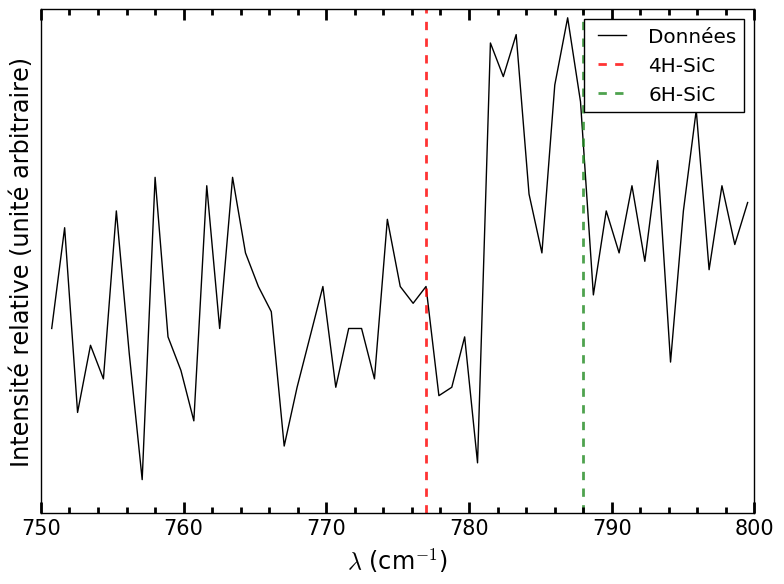
\includegraphics[width=0.8\linewidth]{figures/echantillon1.png}
	\caption{Spectre Stokes pour l'échantillon 1. Le spectre collecté est concentré dans la région $750$ à $800\unit{cm}^{-1}$ pour augmenter la précision des mesures, sachant que les raies distinctives des deux natures possibles de cet échantillon se trouvent dans cette région.}
	\label{fig:e1}
\end{figure}
Les données de la Figure \ref{fig:e1} indiquent que l'échantillon est le polytope 6H-\ce{SiC}. Le pic est légèrement décalé vers la gauche et possède un doublet à $783 \pm 1\unit{cm}^{-1}$. On note de plus qu'un pied s'étend jusqu'à $800\unit{cm}^{-1}$. Ceci est aussi conforme avec le polytope 6H-\ce{SiC}, qui possède un mode $E_1$(PO) à $796.0$\supercite{Burton1998}$\unit{cm}^{-1}$. 
\subsection{Identification de l'échantillon 2}
Le spectre du deuxième échantillon suggère que c'est une gauffre de \ce{InP}. Le pic à $307\pm 5\unit{cm}^{-1}$ se distingue clairement du bruit et correspond au pic attendu de la Table \ref{tab:echantillon}. Le second pic à $351 \pm 5\unit{cm}^{-1}$ est aussi présent à l'intérieur des marges d'incertitudes de l'étude du spectre Raman du \ce{InP} par \citeauthor{Mooradian1966}\supercite{Mooradian1966}. 
\begin{figure}[H]
	\centering
	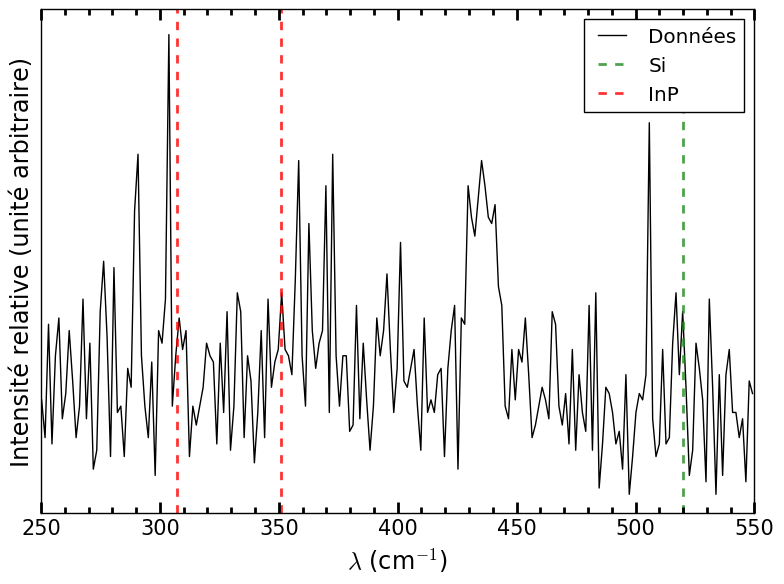
\includegraphics[width=0.8\linewidth]{figures/echantillon2(2).png}
	\caption{Spectre Raman de l'échantillon 2. On y trouve les deux pics attendus (Table \ref{tab:echantillon}) pour \ce{InP}, alors que le pic du \ce{Si} est absent. }
	\label{fig:e2}
\end{figure}


\subsection{Identification de l'échantillon 3}
Le spectre de la Figure \ref{fig:e3} permet d'identifier le $3^e$ échantillion comme étant \ce{TiS2}. Le pic à $230\unit{cm}^{-1}$ se distingue clairement du bruit alors qu'aucun signal n'est présent à la raie attendu pour \ce{SnS2} (Table \ref{tab:echantillon}). 
\begin{figure}[H]
	\centering
	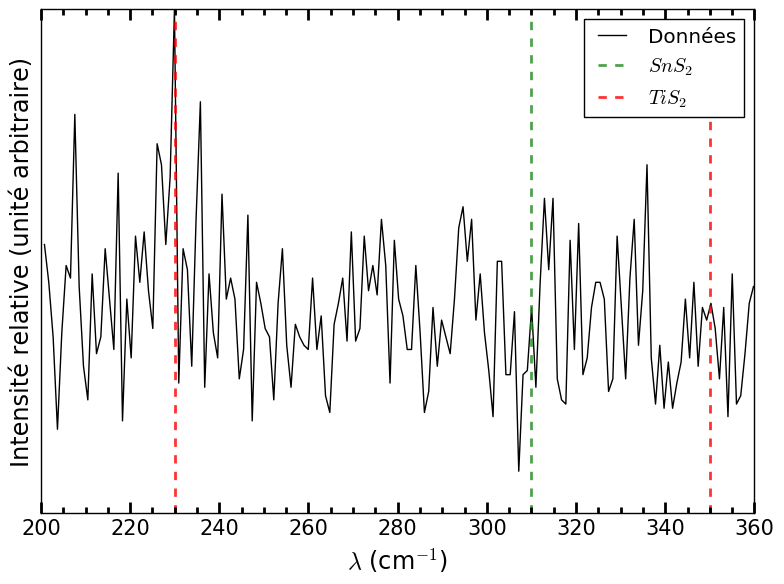
\includegraphics[width=0.8\linewidth]{figures/echantillon3.png}
	\caption{Échantillon 3}
	\label{fig:e3}
\end{figure}
L'intensité des raies Raman du spectre anti-Stokes étaient trop faibles pour les distinguer. Aussi, nous n'avons pas pu mesurer la température de cet échantillon par la méthode de l'équation \ref{eq:temperature}. Cette méthode est plutôt utilisée pour déterminer la température du souffre.

\subsection{Spectre Stokes et anti-Stokes du Souffre}
L'étude du spectre du souffre est une étape commune lors du calibrage d'un montage de spectroscopie Raman. Le spectre de cet élément possède des pics très distinctifs. Dans la Figure \ref{fig:sulfure}, on montre les spectres Stokes et Anti-Stokes d'un crystal rhombique de taille $\sim 3\unit{mm}\times3\unit{mm}\times 3\unit{mm}$. On reconnaît, à partir de l'analyse de \citeauthor{Ward1968}\supercite{Ward1968}, les pics à $\pm218\unit{cm}^{-1}$ et $\pm473\unit{cm}^{-1}$. Ceux-ci sont les plus distinctifs, mais on peut aussi reconnaître le pic à $434\unit{cm}^{-1}$ typique pour le souffre à des températures inférieurs à $200^oC$\supercite{Ward1968}. 
\begin{figure}[H]
	\centering
	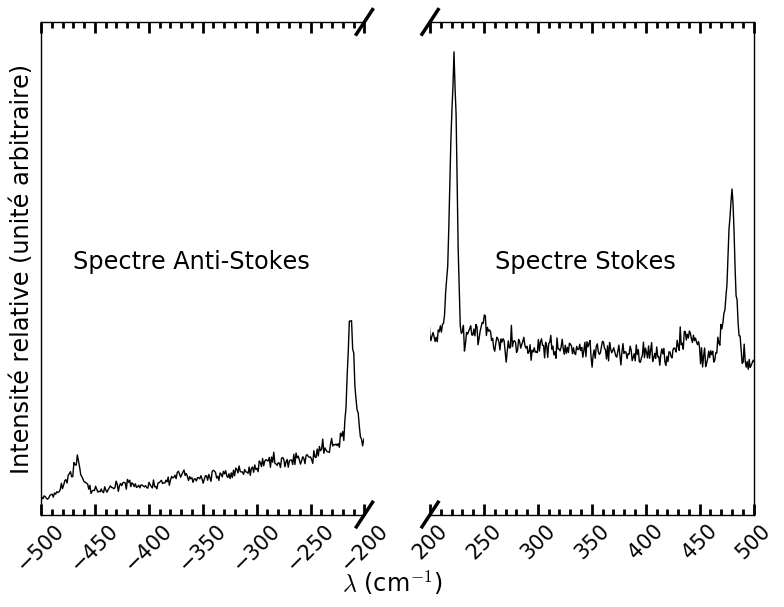
\includegraphics[width=0.8\linewidth]{figures/sulfure.png}
	\caption{Spectre Raman d'un échantillon de souffre. Les pics sont très distinctifs pour cet élément car la diffusion du faisceau principal dans toutes les directions est très forte. }
	\label{fig:sulfure}
\end{figure}
La qualité du spectre anti-Stokes nous permet de mesurer la température du crystal au moment de la mesure à l'aide de l'équation \ref{eq:temperature}. En utilisant les deux phonons visibles dans les deux spectres, on peut estimer la température de l'échantillon par la moyenne des deux résultats . On trouve $$T = 3.3 \pm 2\s\s 10^2K, $$ ce qui est cohérent avec l'apparition du pic à $434\unit{cm}^{-1}$. 


\section{Conclusion}\label{sec:conclusion} % 10 points
Nous avons déterminer la nature des trois échantillons comme étant, en ordre, le polytope 6H-\ce{SiC}, \ce{InP} et \ce{TiS2}. Nous avons aussi déterminé que, pour les fentes minces, le spectroscope possède une résolution inférieure à la résolution idéale prédite par l'équation \ref{eq:dispersion}. Nous avons déterminé que ceci est dû à un élargissement du faisceau par la diffraction de Fraunhofer, ce qui amplifie les aberrations de Siegel. Finalement, nous avons mesurer le spectre du souffre, et déterminé que sa température après quelques minutes d'expositions au laser était $T = 3.3 \pm 2\s\s 10^2K$. 

\printbibliography
%\bibliographystyle{abbvr} 
%\bibliography{raman_scattering_bib}
%\begin{thebibliography}{1}
%\bibitem{ref1} texte de la référence
%\end{thebibliography}

\end{document}
